\documentclass[11pt]{article}
\usepackage[top=1.5cm,bottom=1.5cm,left=1.5cm,right= 1.5cm]{geometry}
%\geometry{landscape}                % Activate for for rotated page geometry
\usepackage[parfill]{parskip}    % Activate to begin paragraphs with an empty line rather than an indent
\usepackage{graphicx}
\usepackage{amssymb}
\usepackage{epstopdf}
\usepackage{amsmath}            
\usepackage{multirow}    
\usepackage{hyperref}
\usepackage{changepage}
\usepackage{lscape}
\usepackage{ulem}
\usepackage{multicol}
\usepackage[usenames,dvipsnames]{color}       
\usepackage{enumerate}
\newcommand{\urlwofont}[1]{\urlstyle{same}\url{#1}}
\newcommand{\degree}{\ensuremath{^\circ}}

\DeclareGraphicsRule{.tif}{png}{.png}{`convert #1 `dirname #1`/`basename #1 .tif`.png}

\newcommand{\soln}[1]{\textcolor{MidnightBlue}{\textit{#1}}}	% delete #1 to get rid of solutions for handouts
%\newcommand{\soln}[1]{ \vspace{3cm} }

\newcommand{\solnMult}[1]{\textbf{\textcolor{MidnightBlue}{\textit{#1}}}}	% uncomment for solutions
%\newcommand{\solnMult}[1]{ #1 }	% uncomment for handouts

\newcommand{\pts}[1]{ \textbf{\textcolor{red}{(#1)}} }	% uncomment for handouts


\begin{document}

{\LARGE \textbf{Midterm 2 Review}}

\begin{itemize}
\item Chp 4: 12, 29, 31, 41
\item Chp 5: 11, 29, 37, 39, 43, 44
\item Chp 6: 2, 4, 14, 26, 33, 38, 40, 44, 49, 51
\item Additional problems:
\begin{enumerate}
 
%

\item Diamond clarity is a quality of diamonds relating to the existence and visual appearance of internal characteristics of a diamond called inclusions, and surface defects called blemishes. Below is a table of the currently used clarity grading scales for diamonds.\footnote{http://en.wikipedia.org/wiki/Diamond\_clarity} 
\begin{center}
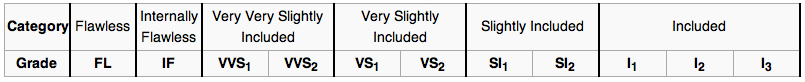
\includegraphics[width=0.8\textwidth]{figures/diamond/diamond_clarity} 
\end{center}
Flawless diamonds are very rare, and so are internally flawless diamonds. In a random sample of 150 diamonds, 5 diamonds are internally flawless (IF).
\begin{enumerate}
\item What methods (theoretical, simulation, or both) can we use to construct a confidence interval for the proportion of diamonds that are internally flawless. Explain your reasoning.
\item Regardless of your answer to part (a), we will construct a confidence interval using a simulation -- bootstrapping. Explain, in your own words, how we can construct a bootstrapping distribution of 100 bootstrap statistics.
\item Below is a bootstrap distribution of 100 bootstrap statistics. What does each dot on this distribution represent? 
\begin{center}
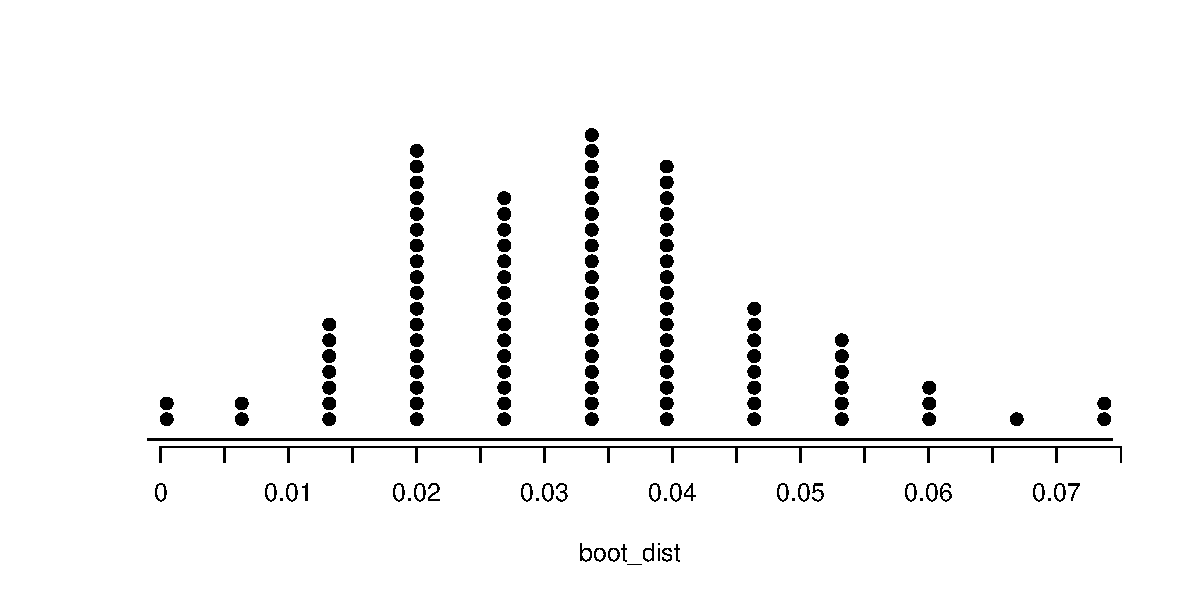
\includegraphics[width=0.6\textwidth]{figures/diamond/diamonds_clarity_boot} 
\end{center}
\item The mean of the above distribution is 0.033 and the standard deviation is 0.015. Calculate the 90\% bootstrap confidence interval using the percentile method as well as the standard error method.
\item Interpret the above confidence interval in context of the question.
\end{enumerate}

\vfill

%

\pagebreak

\item Another criterion that determines the quality of the diamond (and hence its price) is the color. Below is a table of the currently used clarity grading scales for diamonds.\footnote{http://www.allaboutgemstones.com/diamonds\_4cs\_color.html} 
\begin{center}
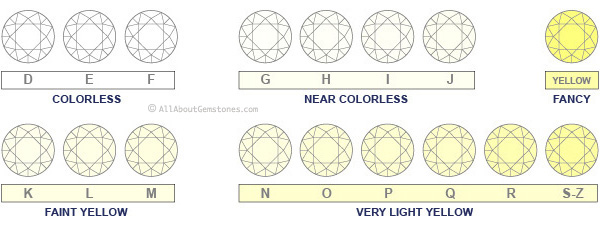
\includegraphics[width=0.6\textwidth]{figures/diamond/diamond_color} 
\end{center}
The table below shows the distribution of clarity and color in the same random sample of 150 diamonds. Clarity is divided into two levels: \texttt{VVS+} which represented very very slightly included or higher, and \texttt{VS-} very slightly included or lower.

\begin{center}
\begin{tabular}{rrr}
  \hline
 & colorless & near colorless \\ 
  \hline
VVS+ &   15 &  15 \\ 
  VS- &  64 &  56 \\ 
   \hline
\end{tabular}
\end{center}

\begin{enumerate}
\item What percent of VVS+ diamonds are colorless?
\item What percent of VS- diamonds are colorless?
\item Write the hypotheses (in words and using notation) for testing if the proportion of colorless diamonds is different between the VVS+ and VS- diamonds.
\item What is the parameter of interest? (in words and using notation)
\item What is the point estimate? (in words and using notation) Calculate this value.
\item Describe, in your own words, how you would conduct a randomization test using index cards.
\item Below is the histogram of a randomization distribution resulting from such randomization test using 100 simulations. What is the conclusion of the hypothesis test?
\begin{center}
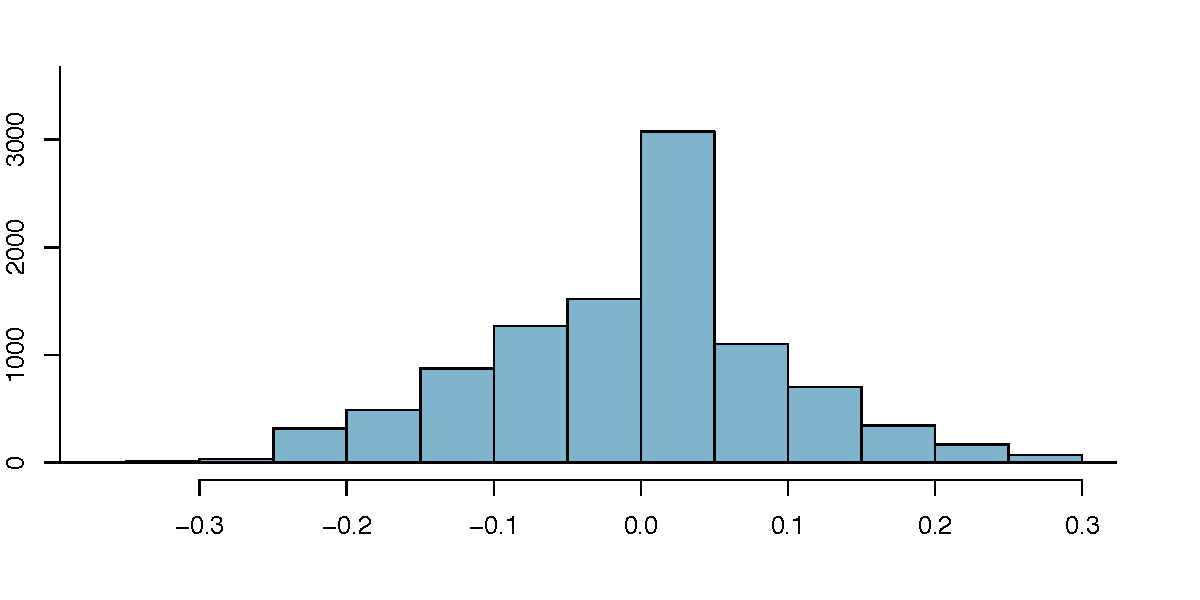
\includegraphics[width=0.7\textwidth]{figures/diamond/diamonds_color_rand} 
\end{center}
\item Would you expect a confidence interval for the difference between the proportions of colorless VVS+ and VS- diamonds to include 0? Explain your reasoning. (Do not calculate a confidence interval, use the result of your hypothesis to answer this question.) 

\end{enumerate}

\end{enumerate}

\end{itemize}

%

\pagebreak

{\large \textbf{\underline{Chapter 4}}}

\begin{enumerate}

\item[4.12]
\begin{enumerate}[(a)]
\item False, inference is made on the population parameter, not the point estimate. The point estimate is always in the confidence interval.
\item False, the strongly right skewed distribution in the sample indicates that the population distribution is most likely right skewed as well, but with a large enough sample size we can assume that the sampling distribution is nearly normal and calculate a confidence interval.
\item False, the confidence interval is not about a sample mean. The true interpretation of the confidence level would be that 95\% of random samples produce confidence intervals that include the true population mean.
\item True, this is the correct interpretation of the confidence interval.
\item True. If we only want to be 90\% confident rather than 95\% confident that we capture the parameter, a smaller interval is required.
\item False, since in calculation of the standard error we divide the standard deviation by square root of the sample size, in order to cut the standard error to a third of what it is now (and hence the margin of error) we would need to sample $3^2 = 9$ times the number of people in the initial sample.
\[ ME_{\text{1/3rd as big}} = z^{\star} \frac{s}{\sqrt{n}} \ \rightarrow \ \frac{1}{3}ME_{original} = z^{\star} \frac{s}{\sqrt{9n}} = z^{\star} \frac{s}{3\sqrt{n}} = \frac{1}{3} z^{\star} \frac{s}{\sqrt{n}}  = \frac{1}{3} ME_{original} \]
\item True, margin of error can be calculated as half the width of the interval:
\[ ME = \frac{89.11 - 80.31}{2} = \frac{8.8}{2} = 4.4 \]
\end{enumerate}

%

\item[4.29]
\begin{enumerate}[(a)]
\item If the null hypothesis is rejected in error, then the regulators concluded that the adverse effect was higher in those taking the drug than those who did not take the drug when in reality the rates are the same for the two groups. 
\item If the null hypothesis is not rejected in error, then the regulators failed to identify that the adverse effect was significantly higher in those taking the drug.
\item Since the regulators used a 5\% significance level, there is at most a 5\% chance that the null hypothesis is rejected in error. So we would be at least 95\% sure that the drug really has an adverse effect. 
\item There is not enough information to tell.
\end{enumerate}

%

\item[4.31]$\:$ \\
\begin{enumerate}[(a)]

\item 
\begin{enumerate}[1.]
\item Independence: The customers are sampled randomly and 70 customers likely make less then 10\% of all happy hour customers at this restaurant, so the observations are independent.
\item Sample size: The sample size is greater than 30.
\item Skew: No information is provided on the skew of the data. We would ask the owner to provide the raw data to check this condition, but for now we will proceed as though this condition is satisfied.
\end{enumerate}

\item $\:$ \\
\begin{minipage}[c]{0.45\textwidth}
\begin{align*}
&H_0: \mu = 18 \\
&H_A: \mu > 18 \\
\: \\
Z &= \frac{19.25 - 18}{ \frac{3.02}{\sqrt{70}} } = 3.46 \\
p-value &= P(\bar{x} > 19.25~|~\mu = 18) \\
&= P(z > 19.25)  \\
&= 1 - 0.9997 = 0.0003
\end{align*}
Since p-value $< \alpha$, reject $H_0$. \\
\end{minipage}
\begin{minipage}[c]{0.05\textwidth}
$\:$
\end{minipage}
\begin{minipage}[c]{0.5\textwidth}
\begin{center}
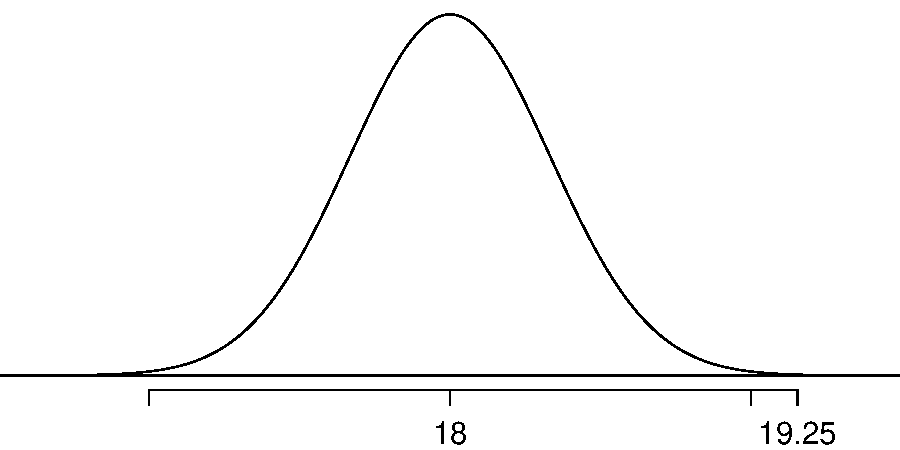
\includegraphics[width=\textwidth]{figures/happyHour} 
\end{center}
There is strong evidence that the average revenue per customer is greater than \$18. 
\end{minipage}

\item The 90\% confidence interval can be calculated as follows:
\begin{align*}
\bar{x} \pm z^{\star} SE &= 19.25 \pm 1.65 \times  \frac{3.02}{\sqrt{70}} \\
&= 19.25 \pm 0.60 \\
&= (18.65, 19.85)
\end{align*}
We are 90\% confident that the true mean revenue per customer is between \$18.65 and \$19.85.

\item Yes, the hypothesis test was significant, yielding evidence that the average revenue per customer has increased when happy hour was extended, and the confidence interval suggest the same as it is above this amount.

\item Even though the increase in average revenue per customer appears to be significant, the restaurant owner may want to consider other criteria before deciding to extend the happy hour as increased revenue per customer does not necessarily mean increased total profits. With a longer happy hour, the revenue over the entire evening may actually drop since lower prices are offered for a longer time. Also, even if the revenue does rise, so might the costs due to increased food and drinks served. A better measure to consider may be an increase in total profits for the entire evening.
\end{enumerate}

%

\item[4.41]
\begin{enumerate}[(a)]
\item The distribution of the lengths of these songs is slightly right skewed to the right, therefore it is not reasonable to use a normal model to estimate this probability. However, we can approximate the probability using the histogram. It appears that there are 350 songs between whose lengths are between 5-6 mins, 100 songs between 6-7 mins, 25 songs between 7-8 mins, 20 songs between 8-9 mins and 5 songs between 9-10 mins. If we let X denote the length of a randomly chosen song, then,
\[ P(X > 5) = \frac{350 + 100 + 25 + 20 + 5}{3000} = \frac{500}{3000} = 0.17 \]
(Answers may vary a little.)

\item Two different answers are reasonable. 
\begin{enumerate}[(1)]
\item CLT conditions are met: \\
Since the population distribution is only slightly skewed to the right, even a small sample size may be sufficient to yield a nearly normal sampling distribution. We also know that the songs are sampled randomly and the sample size is less than 10\% of the population, therefore we can also assume that the length of one song in the sample is independent of another.  We are looking for the probability that the total length of 15 songs is more than 60 minutes. This means that one song on average should last at least $\frac{60}{15} = 4$ minutes.  
Then,
\begin{align*}
\bar{X} &\sim N \left( \mu_{\bar{x}} = 3.45, SE_{\bar{x}} = \frac{1.62}{\sqrt{15}}  \right)  \\
P(\bar{X} > 4) &= P \left( z > \frac{4 - 3.45}{\frac{1.62}{\sqrt{15}}} \right)= P(z > 1.31) = 1 - 0.9049 = 0.0951
\end{align*}

\item CLT conditions are not met: \\
Since the population distribution is not normal, a small sample size may not be sufficient to yield a nearly normal sampling distribution. Therefore, we cannot estimate the probability using the tools we have learned so far.
\end{enumerate}

\item We can now be confident that the conditions are satisfied (see part (b)). Therefore,

\begin{minipage}[c]{0.5\textwidth}
\begin{align*}
\bar{X} &\sim N\left(\mu_{\bar{x}} = 3.45, SE_{\bar{x}} = \frac{1.63}{\sqrt{100}}\right) \\
P(\bar{X} > 3.6 ) &= P\left(z > \frac{3.6 - 3.45}{\frac{1.63}{\sqrt{100}}}\right) \\
&= P(z > 0.92) \\
&= 1 - 0.8212 \\
&=  0.1788
\end{align*}
\end{minipage}
\begin{minipage}[c]{0.5\textwidth}
\begin{center}
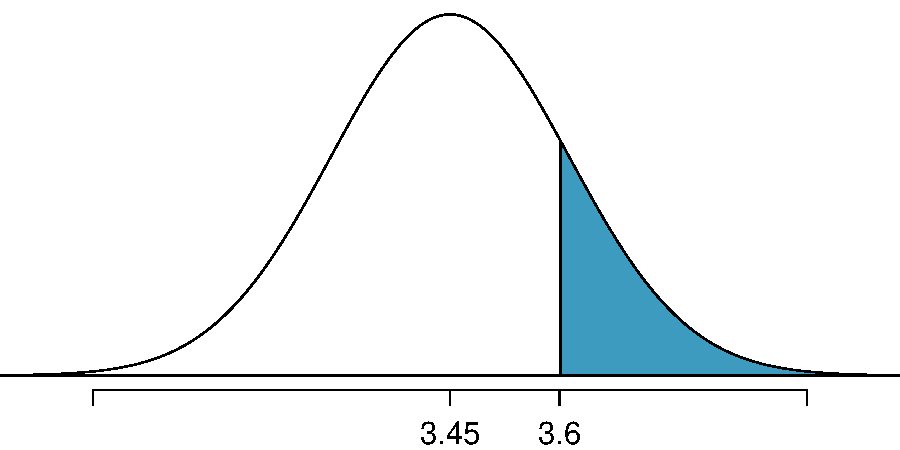
\includegraphics[width=\textwidth]{figures/ipod_n100.pdf}
\end{center}
\end{minipage}
\end{enumerate}
\end{enumerate}
%

\pagebreak

{\large \textbf{\underline{Chapter 5}}}

\begin{enumerate}

\item[5.11]
\begin{enumerate}[(a)]
\item We are 95\% confident that those on the Paleo diet lose 0.891 pounds less to 4.891 pounds more than those in the control group.
\item No, because the value representing no difference between the diets (0) is included in the confidence interval.
\item It would be significant, because this change would just shift the confidence interval over by 1 pound, yielding $CI = (0.109, 5.891)$ which does not include 0.
\end{enumerate}

%

\item[5.29]
\begin{enumerate}[(a)]

\item Chicken that were fed linseed on average weigh 218.75 grams while those that were given horsebean weigh on average 160.20 grams. Both distributions are relatively symmetric with no apparent outliers. There is more variability in the weights of chicken that were given linseed.

\item The hypotheses are $H_0: \mu_{ls} = \mu_{hb}$ and $H_0: \mu_{ls} \ne \mu_{hb}$.

Before calculating the test statistic we should check that the conditions for the sampling distribution of $(\bar{x}_{ls} - \bar{x}_{hb})$ to be nearly normal and the estimate of the standard error to be sufficiently accurate are as follows: 
\begin{itemize}
\item[-] Independence: Chickens are randomly assigned to feed groups, and 12 and 10 $<$ 10\% of all chickens fed linseed and horsebean, respectively. Therefore we can assume that the weights of chicken fed linseed are independent of each other, as well as the weights of chicken fed horsebean.
\item[-] Sample size: Sample sizes are less than 30, so we should use a $t$-test.
\item[-] Skew: The distributions look fairly symmetric.
\end{itemize}

Since population standard deviations are unknown and samples are small, we calculate a T score.

\begin{minipage}[c]{0.5\textwidth}
\begin{align*} 
t_{df} &= \frac{(\bar{x}_{ls} - \bar{x}_{hb}) - (\mu_{ls} - \mu_{hb})}{\sqrt{ \frac{s_{ls}^2}{n_{ls}} + \frac{s_{hb}^2}{n_{hb}} }} \\
&= \frac{(218.75 - 160.20) - 0}{ \sqrt{\frac{52.24^2}{12} + \frac{38.63^2}{10}} } = \frac{58.55}{19.41} = 3.02 \\
df &= min(n_1 - 1, n_2 - 1) = min(11,9) = 9 \\
p-value &= P(|t| > 3.02) \\
0.01 &< p-value < 0.02
\end{align*}
\end{minipage}
\begin{minipage}[c]{0.5\textwidth}
\begin{center}
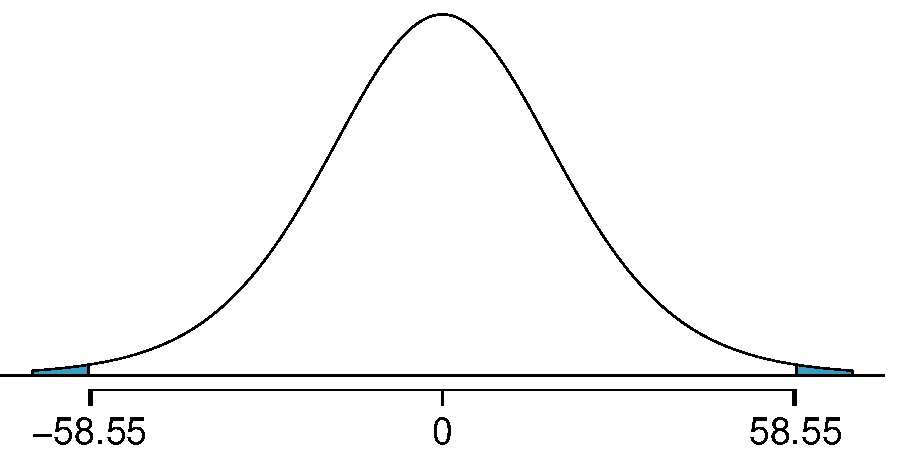
\includegraphics[width=\textwidth]{figures/chicks_ls_hb_pval}
\end{center}
\end{minipage}

Since p-value $<$ 0.05, we reject $H_0$. The data provide strong evidence that there is a significant difference between the average weights of chicken that were fed linseed and horsebean.

\item Type 1, since we rejected $H_0$.

\item Yes, since p-value $>$ 0.01, we would fail to reject $H_0$ and conclude that the data do not provide convincing evidence of a difference between the average weights of chickens that were fed linseed and horsebean.

\end{enumerate}

%

\item[5.37]
The conditions that need to be satisfied for ANOVA are:
\begin{itemize}
\item[-] Independence: Chicks are randomly assigned to feed types (presumably kept separate from one another), therefore independence of observations is reasonable.
\item[-] Approximately normal: The distributions of weights within each feed type appear to be fairly symmetric, with the possible exception of the sunflower group.
\item[-] Constant variance: Based on the side-by-side box plots shown in Exercise~\ref{chicks}, the constant variance assumption appears to be reasonable.
\end{itemize}

The hypotheses are: \\
$H_0$: $\mu_1 = \mu_2 = \cdots = \mu_6$ \\
$H_A$: The average weight varies across some (or all) groups.

$F_{5,65} = 15.36$ and the p-value is approximately 0. With such a small p-value, we reject $H_0$. The data provide convincing evidence that the average weight of chicks varies across some (or all) feed supplement groups.

%

\item[5.39]
\begin{enumerate}[(a)]
\item $H_0$: The mean MET for each group is equal to each other.
\[ \mu_{\le \text{1 cup/week}} = \mu_{\text{2-6 cups/week}} = \mu_{\text{1 cup/day}} = \mu_{\text{2-3 cups/day}} = \mu_{\ge \text{4 cups/day}} \]
$H_A$: At least one pair of means is different.

\item The conditions that need to be satisfied for ANOVA are:
\begin{itemize}
\item[-] Independence: We don't have any information on how the data were collected, so we cannot assess independence. To proceed, we must assume the subjects in each group are independent.
\item[-] Approximately normal: The data are bound below by zero and the standard deviations are larger than the means, indicating very strong strong skew. However, since the sample sizes are extremely large, even extreme skew is acceptable.
\item[-] Constant variance: This condition appears to be met, standard deviations are pretty consistent across groups.
\end{itemize}
In order to proceed with the test we will need to assume independence. 

\item $\:$ \\

\begin{adjustwidth}{-4em}{-4em}
{\scriptsize
\begin{center}
\renewcommand{\arraystretch}{1.25}
\begin{tabular}{lrrrrr}
  \hline
 			& Df 	& Sum Sq		& Mean Sq	& F value	& Pr($>$F) \\ 
  \hline
coffee	 	& \fbox{\textcolor{black}{{\footnotesize 5 - 1 = 4}}}	 & \fbox{\textcolor{black}{{\footnotesize 25575327 - 25564819 = 10508}}} 		& \fbox{\textcolor{black}{{\footnotesize 10508 / 4 = 2627}}} 			& \fbox{\textcolor{black}{{\footnotesize 2627 / 505 = 5.2}}} 	& 0.0003 \\ 
Residuals		& \fbox{\textcolor{black}{{\footnotesize 50739 - 5 = 50734}}} & 25564819 	& \fbox{\textcolor{black}{{\footnotesize  25564819 / 50624 =  505}}} 			&  		&  \\ 
   \hline
Total			& \fbox{\textcolor{black}{{\footnotesize 50739 - 1 = 50738}}} & 25575327
\end{tabular}
\end{center}
}
\end{adjustwidth}

\item Since p-value is low, reject $H_0$. The data provide convincing evidence that the average MET differs between at least one pair of groups.
\end{enumerate}

%

\item[5.43]

\begin{enumerate}[(a)]
\item False, as the number of groups increases so does the number of comparisons and hence the modified significance level decreases.
\item True.
\item True.
\item False, we need observations to be independent regardless of sample size.
\end{enumerate}

%

\item[5.44]

\begin{enumerate}[(a)]
\item False, we conclude that at least one pair of means are different.
\item True.
\item False, it is possible to reject the null hypothesis using ANOVA and then to not subsequently identify differences in the pairwise comparisons.
\item False, the Bonferroni correction requires dividing the original $\alpha$ by the number of pairwise tests to be conducted, not the number of groups. With 4 groups to start with, $k = 4$, the number of pairwise tests will be $K = \frac{k(k-1)}{2} = \frac{4 \times 3}{2} = 6$, and hence the new significance level will be $\alpha^\star = \frac{\alpha}{K} = \frac{0.05}{6} = 0.0083$.
\end{enumerate}

%

\end{enumerate}

%

\pagebreak

{\large \textbf{\underline{Chapter 6}}}

\begin{enumerate}

\item[6.2]
\begin{enumerate}[(a)]
\item TRUE. The success-failure condition is not satisfied
\[ np = 20 \times  0.77 = 15.4~and~ n(1-p) = 20 \times  0.23 = 4.6, \]
therefore we know that the distribution of $\hat{p}$ is not approximately normal. In most samples we would expect $\hat{p}$ to be close to 0.77, the true population proportion. While $\hat{p}$ can be as low as 0 (though we would expect this to happen very rarely), it can only go as high as 1. Therefore, since 0.77 is closer to 1, the distribution would probably take on a left skewed shape. Plotting the sampling distribution would confirm this suspicion.
\item FALSE. Unlike with means, for the sampling distribution of proportions to be approximately normal, we need to have at least 10 successes and 10 failures in our sample. We do not use $n \ge 30$ as a condition to check for the normality of the distribution of $\hat{p}$.
\item FALSE. Standard error of $\hat{p}$ in samples with $n = 60$ can be calculated as:
\[SE_{\hat{p}} = \sqrt{ \frac{p(1-p)}{n} } = \sqrt{\frac{0.77 \times  0.23}{60}} = 0.0543 \]
A $\hat{p}$ of 0.85 is only $Z = \frac{0.85 - 0.77}{0.0543} = 1.47$ standard errors away from the mean, which would not be considered unusual.
\item TRUE. Standard error of $\hat{p}$ in samples with $n = 180$ can be calculated as:
\[SE_{\hat{p}} = \sqrt{ \frac{p(1-p)}{n} } = \sqrt{\frac{0.77 \times  0.23}{180}} = 0.0314 \]
A $\hat{p}$ of 0.85 is $Z = \frac{0.85 - 0.77}{0.0314} = 2.54$ standard errors away from the mean, which might be considered unusual.
\end{enumerate}

%

\item[6.4]
\begin{enumerate}[(a)]
\item TRUE. The success-failure condition is not satisfied
\[ np = 12 \times  0.25 = 4~and~ n(1-p) = 12 \times  0.75 = 8, \]
therefore we know that the distribution of $\hat{p}$ is not approximately normal. In most samples we would expect $\hat{p}$ to be close to 0.25, the true population proportion. While $\hat{p}$ can be as high as 1 (though we would expect this to happen very rarely), it can only go as low as 0. Therefore, since 0.25 is closer to 0, the distribution would probably take on a right skewed shape. Plotting the sampling distribution would confirm this suspicion.
\item TRUE. The minimum sample size that yields at least 10 successes and 10 failures can be calculated as
\[ n = max \left( \frac{10}{0.25}, \frac{10}{0.75} \right) = min(40, 13.3) = 40 \]
We need a sample of at least $n = 40$ to meet the success failure condition.
\item FALSE. Standard error of $\hat{p}$ in samples with $n = 50$ can be calculated as:
\[SE_{\hat{p}} = \sqrt{ \frac{p(1-p)}{n} } = \sqrt{\frac{0.25 \times  0.75}{50}} = 0.0612 \]
A $\hat{p}$ of 0.20 is only $Z = \frac{0.20 - 0.25}{0.0612} = -0.82$ standard errors away from the mean, which would not be considered unusual.
\item FALSE. Standard error of $\hat{p}$ in samples with $n = 150$ can be calculated as:
\[SE_{\hat{p}} = \sqrt{ \frac{p(1-p)}{n} } = \sqrt{\frac{0.25 \times  0.75}{150}} = 0.0354 \]
A $\hat{p}$ of 0.20 is $Z = \frac{0.20 - 0.25}{0.0354} = -1.41$ standard errors away from the mean, which would not be considered unusual.
\item FALSE.  Since $n$ appears under the square root sign in the formula for the standard error, doubling the sample size would decrease the standard error of the sample proportion only by a factor of $\sqrt{3}$.
\end{enumerate}

%

\item[6.14]
\begin{enumerate}[(a)]
\item The hypotheses are as follows:
\begin{itemize}
\item[] $H_0: p = 0.5$ (50\% of Americans think the Civil War is still relevant)
\item[] $H_A: p > 0.5$ (More than 50\% of Americans think the Civil War is still relevant)
\end{itemize}

Before calculating the test statistic we should check that the conditions are satisfied. 
\begin{itemize}
\item[-] Independence:  The sample is random, and $1,507$ $<$ 10\% of all Americans, therefore whether or not one American in the sample thinks the Civil War is still relevant is independent of another.
\item[-] Success-failure:
\[ \text{Successes: } 1,507 \times  0.50 = 753.5 > 10 \checkmark \qquad \text{Failures: } 1,507 \times  0.50 = 753.5 > 10 \checkmark \]
\end{itemize}
Since the observations are independent and the success-failure condition is met, $\hat{p}$ is approximately normal.

The test statistic and the p-value can be calculated as follows:

\begin{minipage}{0.6\textwidth}
\begin{align*}
Z &= \frac{\hat{p} - p_0}{\sqrt{\frac{p_0 (1 - p_0)}{n}}} \\
&= \frac{0.56 - 0.5}{\sqrt{\frac{0.5 \times  0.5}{1,507}}} = \frac{0.06}{0.0129} = 4.65 \\
p-value &= P(\hat{p} >  0.56~|~p = 0.5) \\
&= P(z > 4.65) \approx 0
\end{align*}
\end{minipage}
\begin{minipage}{0.4\textwidth}
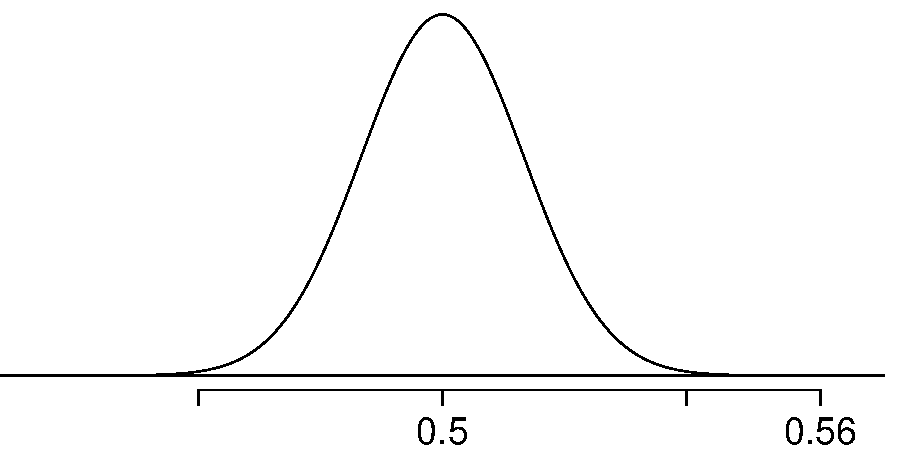
\includegraphics[width=\textwidth]{figures/civilWar_pval}
\end{minipage}

Since the p-value is very small, we reject $H_0$. The data provide strong evidence that the majority of the Americans think the Civil War is still relevant.

\item If in fact only 50\% of Americans thought the Civil War is still relevant, the probability of obtaining a ransom sample of 1,507 Americans where 56\% or more think it is still relevant would be approximately 0.

\item First we need to recheck the success-failure condition using the sample proportion:
\[ \text{Successes: } 1,507 \times  0.56 = 843.92 > 10 \checkmark \qquad \text{Failures: } 1,507 \times  0.44 = 663.08 > 10 \checkmark \]

A 90\% confidence interval can be calculated as follows:
\begin{align*}
\hat{p} \pm z^{\star} \sqrt{\frac{\hat{p} (1 - \hat{p})}{n}} &= 0.56 \pm 1.65 \times  \sqrt{\frac{0.56 \times  0.44}{1,507}} \\
&= 0.56 \pm 1.65 \times  0.0128 = 0.56 \pm 0.02 = (0.54, 0.58)
\end{align*}
We are 90\% confident that 54\% to 58\% of all Americans think that the Civil War is still relevant. This agrees with the conclusion of the earlier hypothesis test since the interval lies above 50\%.
\end{enumerate}

%

\item[6.26]
\begin{enumerate}[(a)]
\item True.
\item False. We are  95\% confident that 7\% to 15\% more college graduates watch The Daily Show than those with a high school degree or lower.
\item False. The confidence level is not about the sample statistic.
\item False. As the confidence level decreases the width of the confidence level decreases as well.
\item True.
\end{enumerate}

%

\item[6.33]
The hypotheses are
\begin{itemize}
\item[] $H_0: p_C = p_T$ (Rate of sleep deprivation is the same for the non-transportation workers and truck drivers.)
\item[] $H_A: p _C \ne p_T$ (Rate of sleep deprivation is different for the non-transportation workers and truck drivers.)
\end{itemize}

Before conducting the hypothesis test, we must first check that the conditions for inference are satisfied.
\begin{itemize}
\item[-] Independence: Both samples are random and from less than 10\% of either population, so observations are independent within each sample. The samples are also unrelated and so are independent.

\item[-] Success-failure: First we need to find the pooled $\hat{p}$ and then use that to calculate the numbers of expected successes and failures in each group.
\begin{align*} 
\hat{p} &= \frac{success_{C} + success_{T}}{n_{C} + n_{T}} = \frac{35 + 35}{292 + 203} = \frac{70}{495} = 0.14 \\
1 - \hat{p} &= 1 - 0.14 =  0.86
\end{align*}
\[ 292 \times  0.14 = 40.88 > 10 \checkmark \qquad 292 \times  0.86 = 251.12 > 10 \checkmark \]
\[ 203 \times  0.14 = 28.42 > 10 \checkmark \qquad 203 \times  0.86 = 174.58 > 10 \checkmark \]
\end{itemize}

Since the observations are independent and the success-failure condition is met, $\hat{p}$ is approximately normal. Next, we calculate the test statistic and the p-value:

\begin{minipage}{0.6\textwidth}
\begin{align*}
\hat{p}_C &= \frac{35}{292} = 0.12 \qquad \hat{p}_T = \frac{35}{203} = 0.17 \\
Z &= \frac{(\hat{p}_C - \hat{p}_T)}{\sqrt{\frac{\hat{p} \hat{q}}{n_C} + \frac{\hat{p} \hat{q}}{n_T}}} = \frac{(0.12 - 0.17)}{\sqrt{\frac{0.14 \times  0.86}{292} + \frac{0.14 \times  0.86}{203}}} = \frac{-0.05}{0.0317} = -1.58 \\
p-value &= P(|z| > 1.58) \\
&= 2 \times 0.0582 = 0.1164 
\end{align*}
\end{minipage}
\begin{minipage}{0.4\textwidth}
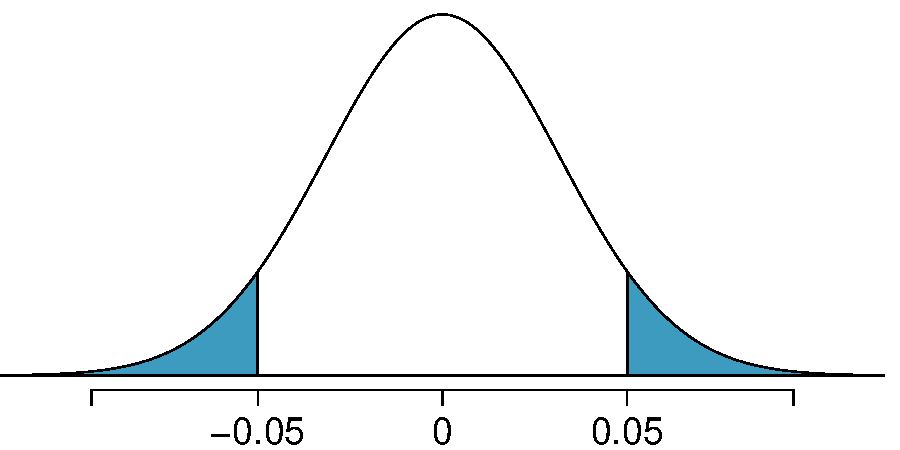
\includegraphics[width=\textwidth]{figures/sleepTransport_pval}
\end{minipage}

Since the p-value is high, we fail to reject $H_0$. The data do not provide strong evidence that the rates of sleep deprivation (defined as getting less than 6 hours of sleep per night) are different for non-transportation workers and truck drivers.

%

\item[6.38]
\begin{enumerate}[(a)]
\item True.
\item True.
\item False. The chi-square distribution is right skewed, and the p-value is defined as $P(\chi^2 > X^2_{observed})$, therefore we only shade the right tail.
\item False. The variability increases as the degrees of freedom increases.
\end{enumerate}

%

\item[6.40]
\begin{enumerate}[(a)]
\item $O_{(1)} = 1,019 \times  0.38 = 387$ \\
$O_{(2)} = 1,019 \times  0.16 = 163$ \\
$O_{(3)} = 1,019 \times  0.40= 408$ \\
$O_{(4)} = 1,019 \times  0.06 = 61$
\item The hypotheses are as follows:
\begin{itemize}
\item[] $H_0$: Distribution of the belief in evolutionary origins of humans has not changed from 2001 to 2010.
\item[] $H_A$: Distribution of the belief in evolutionary origins of humans has changed from 2001 to 2010.
\end{itemize}

\item  $E_{(1)} = 1,019 \times  0.37 = 377$ \\
$E_{(2)} = 1,019 \times  0.12 = 122$ \\
$E_{(3)} = 1,019 \times  0.45= 459$ \\
$E_{(4)} = 1,019 \times  0.06 = 61$
\item Before calculating the test statistic we should check that the conditions are satisfied. 
\begin{itemize}
\item[-] Independence:  The sample is random, and 1,019 $<$ 10\% of all Americans, therefore respondents' answers are independent of each other.
\item[-] Sample size: All expected counts are at least 5.
\item[-] Degrees of freedom: $df = k - 1 = 4 - 1 = 3 > 2$.
\end{itemize}

The chi-squared statistic, the degrees of freedom associated with it, and the p-value can be calculated as follows:
\begin{align*}
X^2 &= \sum \frac{(O - E)^2}{E} =  \frac{(387 - 377)^2} {377} + \frac{(163 - 122)^2} {122} + \frac{(408 - 459)^2} {459} + \frac{(61 - 61)^2}{61} = 19.71 \\
df &= 3 \\
p-value &< 0.001
\end{align*}

Since the p-value $< \alpha$, we reject $H_0$. The data provide strong evidence that the distribution of the belief in evolutionary origins of humans has changed from 2001 to 2010. Since an increase was observed in the response ``Humans evolved, but God had no part in process" there is support for the comment.
\end{enumerate}

%

\item[6.44]
\begin{enumerate}[(a)]
\item Chi-squared test of independence.

\item The hypotheses are:
\begin{itemize}
\item[] $H_0$: Caffeinated coffee consumption and depression in women are independent.
\item[] $H_A$: Caffeinated coffee consumption and clinical are in women dependent/associated.
\end{itemize}

\item Depression: $2607 / 50739 = 0.0514$ \\
No depression: $1 - 0.0514 = 0.9486$

\item $E = \frac{2607 * 6617}{50739} = 339.9854 \approx 340$ \\
$\frac{(O - E)^2}{E} = \frac{(373 - 340)^2}{340} = 3.20$

\item $df = (R - 1) \times (C - 1) = 1 \times 4 = 4$, and $p-value < 0.001$.

\item p-value is small and we reject $H_0$. The data provide convincing evidence to suggest that caffeinated coffee consumption and depression in women are associated.

\item Yes, this is an observational study. Based on this study we can't deduce that drinking more coffee leads to less depression. There may be other factors, lurking variables, that cause decreased depression in women who drink more coffee.

\end{enumerate}

%

\item[6.49]
\begin{enumerate}[(a)]
\item The hypotheses are as follows:
\begin{itemize}
\item[] $H_0: p = 0.69$
\item[] $H_A: p \ne 0.69$
\end{itemize}

\item $\hat{p} = \frac{17}{30} = 0.57$

\item The success-failure condition is not satisfied. Under the null hypothesis, we would expect to have 30*0.69 = 20.7 high school students follow the news but only 30*0.31 = 9.3 to not follow the news.

\item Answers may vary. Each student can be represented with a card. Take 100 cards, 69 black cards representing those who follow the news about Egypt and 31 red cards representing those who do not. Shuffle the cards and draw with replacement (shuffling each time in between draws) 30 cards representing the 30 high school students. Calculate the proportion of black cards in this sample, $\hat{p}_{sim}$, i.e. the proportion of those who follow the news in the simulation. Repeat this many times (e.g. 10,000 times) and plot the resulting sample proportions. The p-value will be two times the proportion of simulations where $\hat{p}_{sim} \le 0.57$. (Note: answers may vary, and in practice we would use a compute to simulate.)

\item The one-tail area is represented by the area shown below in blue. The shaded probability is about $0.005 + 0.02 + 0.035 + 0.075 = 0.135$, meaning the two-sided p-value is about 0.27. Your p-value may vary slightly since it is based on a visual estimate in this exercise.

\begin{minipage}[c]{0.5\textwidth}
Since p-value is greater than 0.05, we fail to reject $H_0$. The data do not provide strong evidence that the proportion of high school students who followed the news about Egypt is different than the proportion of American adults who did. 
\end{minipage}
\begin{minipage}[c]{0.5\textwidth}
\begin{center}
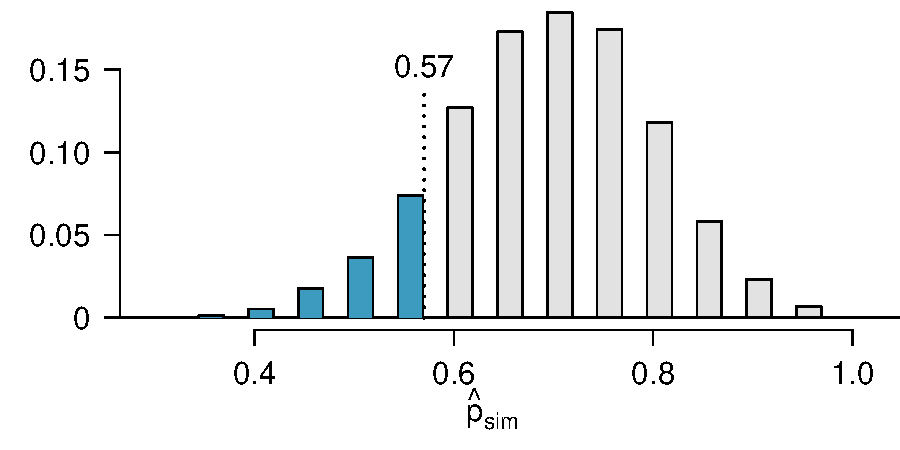
\includegraphics[width= 0.9\textwidth]{figures/egyptSoln}
\end{center}
\end{minipage}
\end{enumerate}

%

\item[6.51]
\begin{enumerate}[(a)]
\item The hypotheses are as follows:
\begin{itemize}
\item[] $H_0: p_{pr} = p_{con}$
\item[] $H_A: p_{pr} \ne p_{con}$
\end{itemize}

\item $\frac{5}{20} - \frac{15}{25} = -0.35$
\item The p-value is represented by the area shown below in blue. In 143 out of the 10,000 simulations differences under the null hypothesis was less than or equal to 0.35. Doubling the one tail, the p-value is about 0.03. (Note that students may have approximate results.)

\noindent \begin{minipage}[c]{0.5\textwidth}
Since p-value is low, we reject $H_0$. The data provide strong evidence that people react differently under the two scenarios.
\end{minipage}
\begin{minipage}[c]{0.5\textwidth}
\begin{center}
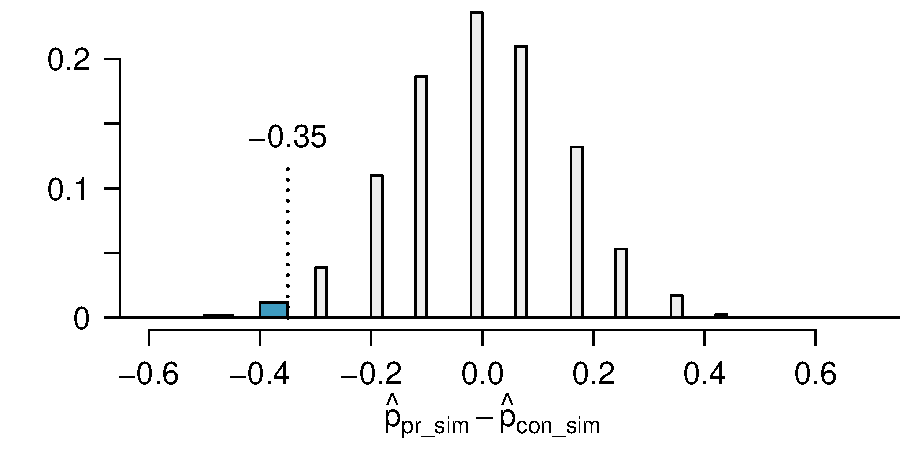
\includegraphics[width= 0.9\textwidth]{figures/socExpSoln}
\end{center}
\end{minipage}
\end{enumerate}

\end{enumerate}

%

\pagebreak

\textbf{Additional problems:}

\begin{enumerate}

\item
\begin{enumerate}
\item We know that the sample is random and can safely assume 150 $<$ 10\% of all diamonds, so we can assume that one diamond in the sample is independent of another. In this sample there are 5 internally flawless diamonds (successes) and this is less than 10, we couldn't use theoretical methods, and must use simulation methods to construct this confidence interval.

\item Sample, with replacement, 150 diamonds from the original sample and record the proportion internally flawless diamonds in this bootstrap sample. Repeat this 100 times and plot the distribution of the bootstrap proportions. 

\item Each dot represents a bootstrap proportion - proportion of internally flawless diamonds in a bootstrap sample of 150 from the original sample. 

\item \textit{Percentile method:} The bounds of the confidence interval mark the middle 90\% of the bootstrap distribution. Since the distribution is comprised of 100 bootstrap proportions, we find the cutoff points that mark the lower and upper 5\% (5 points on each end) of the distribution: (0.013, 0.06). \\
\textit{Standard error method:} $0.033 \pm 1.65 * 0.015 =  (0.00825, 0.05775)$.

\item We are 90\% confident that roughly 1.3\% to 6\% of all diamonds are internally flawless (based on the percentile method).
\end{enumerate}

%

\item 
\begin{enumerate}
\item $15 / (15 + 15) = 0.5$
\item $64 / (64 + 56) = 0.533$
\item $H_0: p_{VVS+} = p_{VS-}$; Proportions of colorless VVS+ and VS- diamonds are equal. \\
$H_0: p_{VVS+} \ne p_{VS-}$; Proportions of colorless VVS+ and VS- diamonds are different.
\item Difference between the population proportions of colorless VVS+ and VS- diamonds;  $p_{VVS+} = p_{VS-}$
\item Difference between the sample proportions of colorless VVS+ and VS- diamonds;  $\hat{p}_{VVS+} = \hat{p}_{VS-} = 0.5 - 0.533 = -0.033$
\item Start with 150 index cards, 79 that say colorless and 71 near colorless on them. Shuffle these cards and split them into two groups, one of size 30 for VVS+ and another of size 120 for VS-. Calculate the proportions of colorless diamonds (cards) in each group and find the simulated difference $(\hat{p}_{VVS+} - \hat{p}_{VS-})$. Repeat this may times and calculate the proportion of simulations where the difference between the two proportions is at least 0.033, in either direction since the alternative hypothesis is two sided. 
\item 0.033 is not an unusual observation based on this randomization distribution. The p-value this yields would be pretty high, resulting in failure to reject the null hypothesis. The data do not provide convincing evidence that the proportion of colorless diamonds is different for VVS+ and VS- diamonds.
\item Since we failed to reject $H_0$ which sets the difference between the two proportions to 0, we would expect the confidence interval to include 0.

\end{enumerate}

\end{enumerate}

%

\end{document}